% Drawn for this paper. Left: the convex hull of four value vectors, with several
% admissible head outputs inside it; the cage idea is Richter and Wattenhofer's,
% the drawing is ours. Right: the readout's box against the counts it must reach,
% plotted from the formulas, not from any measurement.
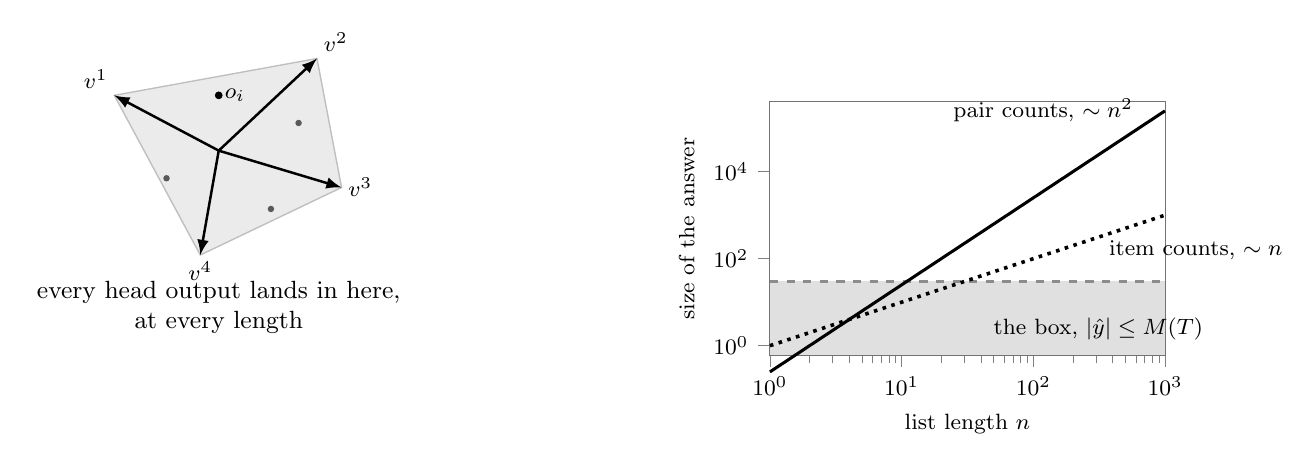
\begin{tikzpicture}
\begin{scope}[scale=0.78]
  \coordinate (O)  at (0,0);
  \coordinate (V1) at (-1.7, 0.9);
  \coordinate (V2) at ( 1.6, 1.5);
  \coordinate (V3) at ( 2.0,-0.6);
  \coordinate (V4) at (-0.3,-1.7);
  \fill[black!8,draw=black!25,line width=0.5pt] (V1) -- (V2) -- (V3) -- (V4) -- cycle;
  \foreach \v/\lab/\pos in {V1/{v^{1}}/{above left}, V2/{v^{2}}/{above right},
                            V3/{v^{3}}/{right}, V4/{v^{4}}/{below}}
    \draw[-latex,line width=0.9pt] (O) -- (\v) node[\pos,font=\footnotesize,inner sep=2pt] {$\lab$};
  \fill[black!65] (-0.85,-0.45) circle (1.5pt);
  \fill[black!65] ( 1.30, 0.45) circle (1.5pt);
  \fill[black!65] ( 0.85,-0.95) circle (1.5pt);
  \fill (0.00,0.90) circle (1.8pt) node[right,font=\footnotesize,inner sep=2pt] {$o_i$};
  \node[font=\small,align=center] at (0,-2.55) {every head output lands in here,\\at every length};
\end{scope}
\begin{scope}[xshift=7.0cm,yshift=-2.6cm]
\begin{axis}[
  width=6.6cm, height=4.8cm,
  xmode=log, ymode=log, log basis x=10,
  domain=1:1000, samples=80,
  xmin=1, xmax=1000, ymin=0.6, ymax=4e5,
  ytickten={0,2,4},
  xlabel={list length $n$}, ylabel={size of the answer},
  tick label style={font=\footnotesize}, label style={font=\footnotesize},
  tick align=outside, tick pos=left,
  axis line style={black!55},
  clip=false,
]
% the box the readout can reach: fixed by the weights, not by n
\fill[black!12] (axis cs:1,0.6) rectangle (axis cs:1000,30);
\draw[black!45,dashed,line width=0.8pt] (axis cs:1,30) -- (axis cs:1000,30);
\node[anchor=west,font=\footnotesize,inner sep=2pt] at (axis cs:45,2.4)
  {the box, $|\hat{y}|\le M(T)$};
\addplot[black,line width=1.1pt] {x*x/4};
  \node[anchor=south east,font=\footnotesize,inner sep=1.5pt,yshift=1pt]
    at (axis cs:620,96100) {pair counts, $\sim n^{2}$};
\addplot[black,dotted,line width=1.3pt] {x};
  \node[anchor=north west,font=\footnotesize,inner sep=1.5pt,xshift=1pt]
    at (axis cs:330,330) {item counts, $\sim n$};
\end{axis}
\end{scope}
\end{tikzpicture}
